\documentclass{article}
\usepackage{amsmath,amsfonts,amssymb,graphicx,color,float}
\begin{document}
\section*{2 Filters in time domain and the Fourier domain}
For a thorough discussion of the effects that a general filter has on a time series, a valuable diagnostic is the frequency response of that filter. This frequency response is the Fourier transform of the filters factors. The Fourier transform is often also referred to as the Fourier spectrum.
\section*{\small 2.1 The Fourier transform}
The Fourier transform Y $(\omega)$ of a function of time \textit{y}(\textit{t}) is:
\begin{equation}
Y (\omega)\equiv \mathcal{F} (\textit{y})= \int dt \ e^{i \omega t} y(\textit{t})
\end{equation}
in which $\omega$ is the frequency of a signal, related to the period \textit{P} by:
\begin{equation}
\omega = \frac {2\pi}{P}
\end{equation}
This paper will refer to \textit{y$_{ti}$} with \textit{y$_t$}. Formula (1) makes use of the relation between exponential and sinusoidal functions:
\begin{equation}
e^{i \omega t} \equiv \cos(\omega t) + i \sin(\omega t)
\end{equation}
If the function \textit{y}(\textit{t}) is only known at discretely sampled times \textit{t$_i$}, which are regularly spaced, a discrete version of the Fourier transform can be defined as well, where the integrals are replaced by summations with appropriate weights for each of the samples \textit{y$_t$}, as follows:
\begin{equation}
\mathcal{F}(y) = \sum_t  \ e^{i \omega t} y(\textit{t})
\end{equation}
For the Fourier transform there is also an inverse operation.
\begin{equation}
y(\textit{t}) = \mathcal{F}^{-1} (Y) = \frac {1}{2 \pi} \ \int d\omega \ e^{-i \omega t} Y(\omega)
\end{equation}
Since there are particularly efficient algorithms (the Fast Fourier transforms or FFTs) for computing discrete Fourier transforms if the number of samples is exactly a power of 2, normally time series are truncated to an appropriate length or padded out symmetrically with appropriate averages values in order to get the number of samples to satisfy this criterion. A useful reference for FFT implementations and their properties is Press et al. (1992).\\One property of the Fourier transforms, whether continuous or discrete, that will be useful for the further discussion, is that they are linear operations, and therefore so are the inverse operations. Linearity implies that the Fourier transform of the sum of functions \textit{y}(\textit{t}) and \textit{z}(\textit{t}) is the sum of their Fourier transforms (Bracewell, 1965):
\begin{equation}
\mathcal{F}(\textit{a} y + \textit{b} z) = \textit{a} \ \mathcal{F}(y)+ \textit{b} \ \mathcal{F}(z)
\end{equation}
where \textit{a} and \textit{b} can be any constants.\\Of particular importance when carrying out discrete Fourier transforms is a limitation that is imposed by the sampling cadence. Indeed, with a finite cadence of sampling, with time interval $\Delta t$ , it is impossible to detect any periodic signal with a frequency that is higher than the Nyquist frequency. This frequency is:
\begin{equation}
\omega_{N_{yq}} = \frac {\pi}{\Delta t}
\end{equation}\\
{\color{red}The Nyquist frequency is related somehow to the number of considered periods T, in the following manner:
\begin{equation*}
\begin{split}
T=N\Delta_{t,}\quad \Delta_{t}=\frac{T}{N},\quad \text{and so}: \quad \omega_{Nyq}=\frac{\pi N}{T}
\end{split}
\end{equation*}
where N is the number of observations.}\\
A discretely sampled finite time series can be represented without loss of information by its discretely sampled Fourier transform. Since the Fourier transform or spectrum is in general complex valued, the number of sampling points required is only half the number of points in the time series. If a standard FFT is applied on a time series, these sampling points are uniformly spaced over the frequency interval\ $\in [0,\omega_{Nyq}$].\\The reason for discussing Fourier transforms in the context of filtering a time series is that filtering in the time domain corresponds to a particularly simple operation in the frequency domain. In general, filtering in the time domain of a regularly sampled time series can be written in the form of a weighted average:
\begin{equation}
\tilde {y_t} = \sum\limits_{k=-m}^{n} \textit{w$_k$}\textit{y$_{t+k}$}
\end{equation}
where the weights \textit{w$_k$} are the filter’s factors. This is a general form, allowing for asymmetric filtering. For instance, in causal filters, $n=0$, so that only information from the previous and present observations of a time point is used and none from the successive. While \textit{m} and/or \textit{n} could in principle be infinite, this has no practical purpose in the current context. Also, in the context of seasonal filtering it is more usual to employ symmetric filters so that not only $m=n$ but also $w_{-k} = w_k$. Often an additional property imposed is that $\sum w_k = 1$, but in the applications at hand this is not always used. \\ The equation (8) above is known as a convolution in the time domain of the function \textit{y} and the function \textit{w}, in which the latter is simply the set of averaging weights interpreted as (samples of) a function of time. It can be demonstrated that the Fourier transform of the convolution of two series in the time domain is identical to the product of the Fourier transforms of the two series (cf. Bracewell, 1965). Therefore the Fourier transform of the filtered time series $\textit{\~ y}$ can be calculated as the product of the Fourier transform of the original time series and the Fourier transform of the filter function \textit{w}.
\begin{equation}
\mathcal{F}(\tilde {y}) = \mathcal{F}(y * w) = \mathcal{F}(y)\mathcal{F}(w)
\end{equation}
in which the * indicates the convolution of functions. Multiplication is a much more straightforward operation than calculating the above running averages of (8), and in the frequency domain it is also more straightforward to see the effect of a filter on signals with a particular frequency or period. In the paper of Dagum et al. (1996) the properties in the frequency domain of many of the filter choices of the X11-ARIMA package are discussed in details, which remain valid also for the more recent X12 implementations.\\ This suggests an alternative approach to constructing a set of averaging weights, namely by starting with a some desirable properties of the filter in the Fourier domain, and then inverse transforming to obtain the appropriate weights \textit{w$_k$}.
\subsection*{\small 2.2 Designing an improved filter}
Determining the effect that a particular set of weights \textit{w} has in the frequency domain is useful in the design of a set of weights that is in some sense ``optimal''. In practical operations of eg. Statistics Netherlands the intention is to regularly publish or update seasonal adjusted time series and perhaps also seasonal influences of a time series. In this case it may be more useful to carry out the running average in the time domain, rather than Fourier transforming the entire time series, carrying out the multiplication in the frequency domain and subsequently inverse transforming again. Useful discussions of the spectral analysis of time domain filters can be found for instance in Grether \& Nerlove (1970), Shumway \& Stoffer (2011) and Findley \& Martin (2006).\\In designing the weights \textit{w} it is advisable  to have the total extent of non-zero values \textit{w} as limited as feasible, ie. to make \textit{m} and \textit{n} in equation (8) as small as possible.
\begin{equation}
w_k \equiv 0 \ \ \ \ \forall |k| > max(m,n)
\end{equation}
\\The reason for this is that when updating the published seasonal adjusted time series, only the most recent samples need to be flagged as provisional, whereas further back beyond the $m^{th}$ sampled point in the past the seasonal adjusted series can be considered final, because by design it can no longer change in any regular update.\\A separate desirable feature is for the Fourier transform of \textit{w} to have zero imaginary part, $\mathfrak{F}(W) = 0$, so that the phase of periodic signals is unaffected by the filtering operations.\\For the Fourier transform of \textit{w} to be entirely real, the weights \textit{w} need to be symmetric around 0. For this reason the design will focus on symmetric weights for which:
\begin{equation}
w_{-k} = w_k
\end{equation}
Another requirement is that the long-term average of the seasonal component has to be equal to 0. Translated to the frequency domain, this means that the value of the Fourier transform of the seasonal component at $\omega=0$ must be equal to 0. The Fourier transform of the original time series can have any value, so by making use of equation (9) it can be seen that this requirement can be met if the Fourier transform $W(\omega)$ of the weights \textit{w} for isolating the seasonal component is equal to 0 at $\omega=0$.  Translating the requirement $W(0)=0$ back to the time domain yields the simple constraint that:
\begin{equation}
\sum \limits_{k=-n}^n w_k \equiv 0
\end{equation}
If the weights \textit{w} are designed to determine the seasonal component, the \textit{trend+ cycle+noise} can be obtained by subtracting the seasonal component from the original time series. This is the case of the set of filter proposed in here. The linearity property (5) ensures that such additions and subtractions in the time domain are treated identically in the frequency domain. If one has a filter W($\omega$) in the frequency domain which is designed to extract seasonal behaviour from a time series, then the filter 1 - W produces a time series with just the \textit{trend+cycle+noise}. This implies that there is an additional desirable property or (soft) constraint for the values $W_k$ in the frequency domain which is that:
\begin{equation}
-\epsilon < W_k < 1+\delta
\end{equation}
In which $\epsilon$ and $\delta$ are as small as feasible given the other constraints. While ideally $\epsilon=0$ and $\delta=0$, in practice with a finite set of filter weights \textit{w} satisfying (10), this may not be achievable. This implies that if the dynamic range of the original time series is very high (ie. the height $h_f$ of a peak in the Fourier transform of the time series is very large) there may still be undesirable remaining seasonal signal in the filtered time series, because $\delta h_f$ and/or $\epsilon h_f$ are not sufficiently small.\\The standard filtering involved in procedures such TRAMO/SEATS and X-13-ARIMA imply an assumption or idealisation that the seasonal component(s) in the time series are perfectly periodic and repeat identically from one year to the next. If this were indeed the case, then it would be perfectly adequate to design weights that eliminate signal at very specific frequencies that are integer values in the units of cycle/years. The weights of this standard approach, when Fourier transformed, produce the diagram of figure 2. It clearly shows notches precisely at integer multiples of 1 cycle/year, broadened because of the finite resolution of the sampling in the frequency domain.\\
The problem with standard filtering is that signal that is not precisely at these frequencies but in-between, is not included in the seasonal effect. For a real time series this genuinely causes issues because in practice also the ``envelope'' of the seasonal effect is subject to long term changes. The seasonal pattern may qualitatively be very similar from year to year but most often it will not be completely identical from one year to the next: eg. the amplitude may be well modulated by effects similar to those that determine long-term trends or economic cycles. Such long term effects on seasonal patterns have a signature in the frequency domain: strong peaks at integer multiples of one cycle/year will be substantially broadened, and therefore produce signals at frequencies where the filter corresponding to the naive design of the standard procedures will not include them in the seasonal component and, therefore, also not extract them from the \textit{trend+cycle+noise} component.\\For this reason it is more suitable for real time series to design a filter that ``removes'' all signal in a band between frequencies of around one cycle/year ie. between $\sim$ 1/12 cycle/month and $\sim$ 5/12 cycle/month. In the context of smoothing a monthly input, the frequency domain $\Omega=(0<\omega<0.5)$ can be portioned in two main intervals: (1) $\Omega=(0 \leq \omega \leq 0.06)$ associated with cycles of 16 months or longer attributed to the signal (trend/cycle) of the series and (2) $\bar{\Omega}=(0.06 < \omega < 0.5)$ (the signal of higher frequencies up to the Nyquist frequency) corresponding to short cyclical fluctuations and the noise. It is in particular for the signal in this range that the full strength of the auto-regressive modelling offered, for instance, by X-13-ARIMA can be employed to further characterise the time series for in-depth analysis. Figure 2 shows an example of what can be achieved in terms of a filter designed to separate out signal in a band of frequencies between $\sim$ 1/12 cycle/month and $\sim$ 5/12 cycle/month. Evidently this is not completely unique, in the sense that slight variations in this frequency response that are visually almost un-noticable, would have some effects on the weights \textit{w}.
\begin{figure}[H]
  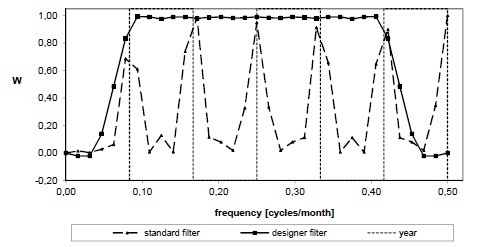
\includegraphics[width=\linewidth]{../images/capitolo2/filters.jpg}
 {\textbf{\scriptsize Figure 2: The band-pass filter designed for seasonal adjustment. Dashed line indicates the standard filter. Small dashed line indicates integer multiples of 1 cycle/year.}}
\end{figure}
The weights \textit{w} that correspond to this filter of figure 2 are shown to 7 digits precision in table 1. The weights \textit{w$_k$} for all the odd values of \textit{k} are identically equal to 0, as are the weights for $ k>18$. This set of weights satisfies the various constraints mentioned in this section. The additional property that the weights are zero for all odd values of\textit{ k} produces an additional advantage: the high frequency section of the spectrum can be determined in a very simple second step, which is evidently statistically independent. If \textit{y} is the time series from which the seasonal component has been removed with the above filter, then the high frequency component \textit{h} is obtained by taking:
\begin{equation}
h_i = (2 \tilde{y_i} - \tilde{y_i} - \tilde{y}_{i+1})/4
\end{equation}
Whereas the \textit{trend+cycle} time series \textit{c} (without high frequency contributions) is obtained from:
\begin{equation}
c_i = (2\tilde{y_i}+\tilde{y_i}+\tilde{y}_{i+1})/4
\end{equation}
With the weights of table 1 it is clear that after 18 months any seasonal adjusted time series \textit{y} will not change, when using this filter alone.
\begin{table}[h!]
\centering
\begin{tabular}{r r}
k & $w_k=w_{-k}$\\
\hline
0 & 0,7358026\\
2 & -0,2219532\\
4 & -0,1504270\\
6 & -0,0659661\\
8 & 0\\
10 & 0,0309203\\
12 & 0,0302373\\
14 & 0,0143577\\
16 & 0\\
18 & -0,0050703\\
\hline
\end{tabular}
\end{table}
\\{\textbf{\scriptsize Table 1: Filter weights for a band-pass filter designed to extract seasonal behaviour from a time series.}}
\bigskip
\\Given that applying this filter to any given time series is as straightforward as the more standard filtering steps (such as applying Henderson filter for smoothing a time series) there is no fundamental difficulty in incorporating this filtering choice in the standard packages that are currently widely available. By doing this, for instance, with the X-13-ARIMA package, all the other tools that this package offers are still available. In particular, the high-frequency noisy term \textit{h} would be the most interesting target for further ARIMA modelling. \\A possible alternative is to pre-process time series with this filter, and this is exactly what is going to be done in the next chapter. There is no loss of information in this pre-processing step since the seasonal factor and the \textit{trend+cycle+noise} series are both available and their sum is identical to the original time series. One or the other of these time series can then be provided as input for the standard packages (in this case, JDemetra+) to be able to use the extensive toolset of those packages for more detailed analyses of the character and causality of the seasonal behaviour. Such more in-depth analyses could be ``off-line'' and would not interfere with the normal publishing schedules of the original and seasonal adjusted time series.
At last, figure 3 plots the two mentioned set of filters in time domain representation, comparing them with the function of the designed one.
 \begin{figure}[H]
  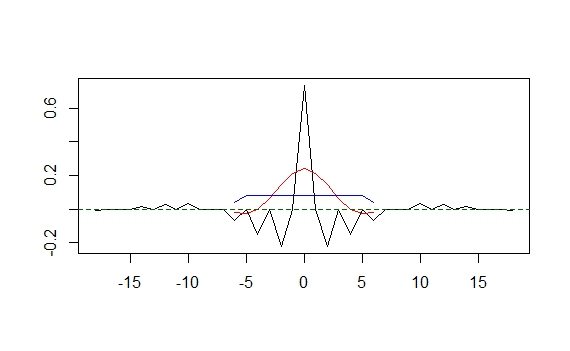
\includegraphics[width=\linewidth]{../images/capitolo2/henderson_designed_ma.jpeg}
  {\textbf{\scriptsize Figure 3: Time-domain representation of different filters. Black line is the designed filter, ranging in a [-18:18] terms width; red line indicates the Henderson 13-terms filter and blue line indicates the 13-terms seasonal moving average filter}}
\end{figure}
\section*{\small 2.3 Periodogram}
Time series, independently of the phenomenon they represent, are generally presented in the time domain. Another interesting view of the same series is in the frequency domain, considering that any stationary time series can be expressed as a combination of sinusoidal functions, thanks to the Fourier transform. The frequency domain tool used by time series analysts is called spectrum, and its representation is called periodogram. It is possible to obtain it as follows:
\begin{equation}
y_t = \sum\limits_{i=1}^{\frac{n}{2}}[\beta_{1_{i}}\cos(2\pi\omega_{i}t) + \beta_{2_{i}}\sin(2\pi\omega_{i}t)]
\end{equation}
The $\beta$'s work as regression parameters, obtained from: $\beta_{1_{i}}=A_{i} \cos(\phi_{i})$ and $\beta_{2_{i}}=-A \sin(\phi_{i})$, where $\phi$ is called the phase; it determines the starting point (in degrees) for the cosine wave. A is the amplitude.
\\The spectral analysis investigates the frequency domain representation of the series to determine how important cycles of different frequencies are in accounting for the behaviour of \textit{y$_t$}. Therefore, the periodogram is useful to identify the dominant periods (or frequencies) of a time series. Peaks in a periodogram indicate frequencies of cyclical movements with a certain periodicity. The periodicity \textit{P} of a phenomenon is related to its frequency $\omega$: $P=2 \pi / \omega$. It means that for a monthly series, seasonal frequencies are $\pi/6$, $\pi/3$, $\pi/2$, $2\pi/3$, $5\pi/6$ and $\pi$, and they correspond to 1, 2, 3, 4, 5 and 6 cycles per year (for quarterly sampled series, the two seasonal frequencies are $\pi/2$; one cycle per year, and $\pi$; two cycles per year).\\The trading day frequency is 0.348, since a daily component which repeats every seven days goes through 4.348 cycles in a month of average length 30.4375 days. It means, then, that 0.348 is the trading days frequency for monthly sampled time series, considering the average length of a year (365.25 days). Actually, the original trading days frequency (4.348) is higher than the Nyquist frequency. If any signal has a frequency higher than the $\omega_{N_{yq}}$, it is an aliasing signal, i.e. it is indistinguishable from a lower-frequency signal. When this happens, the signal “appears” with much lower $\omega$. Consequently, $\omega=4.348$ appears as 0.348.\\A time series with a strong seasonal component should have peaks at the seasonal frequencies, while a seasonally adjusted time series should not have any peaks at those frequencies. Moreover, the presence of the trend component is always evidenced by a peak at frequency zero and so, when a periodogram has high values at low frequencies, it means that the long-term component (the trend) is dominating the series. On the contrary, if high values of the periodogram concentrate more at high frequencies, the time series is rather trendless and has a significant irregular component.\\JDemetra+ contains different spectral diagnostics. First, it is possibile to have a spectral plot of the raw time series, obtained (by default) after a first difference operation to get the data stationary. Indeed, non-stationarity of the series could lead to a misinterpretation of the periodogram.  One other issue is related to the presence of outliers, since they can influence the interpretation of the periodogram as well. This is why a pre-transformation of data is advisable, as done by both TRAMO/SEATS and X-13-ARIMA.  As is visible from figure 3, in JDemetra+ the seasonal frequencies are marked as grey vertical lines, while the violet lines represents the trading day frequency.\\
\begin{figure}[h!]
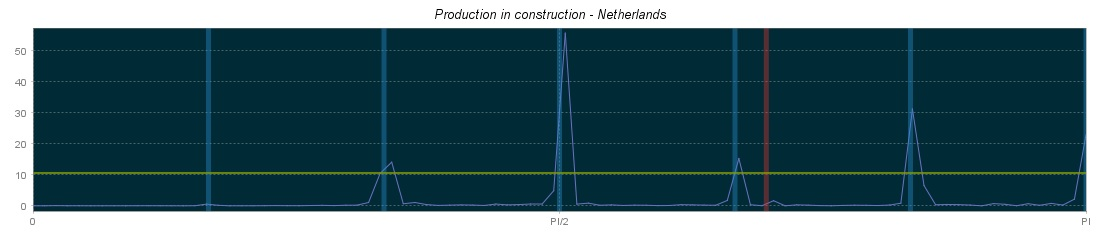
\includegraphics[width=\linewidth]{../images/capitolo2/raw.jpg}
\centering
{\textbf{\scriptsize Figure 4: JDemetra+ representation of a periodogram}}
\end{figure}
\\In addition to the ‘raw’ periodogram, once the seasonal adjustment procedure has been carried out, JDemetra+ offers some spectral diagnostics. In particular, it is possible to check periodograms of the seasonally adjusted series, residuals and irregular component. Further details will be given in the next chapter.
\end{document}

